\documentclass{article}

% Packages
\usepackage[utf8]{inputenc} % For modern characters
\usepackage{microtype} % For sexy kerning
\usepackage{mathtools} % For math stuff
\usepackage{amssymb} % For math symbols
\usepackage{tabularx} % For making tables
\usepackage{fancyhdr} % Use a header
\usepackage{pdfpages} % For including a graphics path

% Set the margins to limit whitespace
\usepackage[scale=0.8, top=1in, bottom=1in]{geometry}

% Other front matter
\graphicspath{ {img/} } % Put all images in img/
\newcommand{\code}[1]{\texttt{#1}} % More readable for writing inline code.
\newcommand{\p}[1]{\paragraph{#1}} % Easier to type out for paragraph command
\newcommand{\addsection}[1]{\addcontentsline{toc}{section}{#1}} % content lines
\newcommand{\addsubsection}[1]{\addcontentsline{toc}{subsection}{#1}} % content line
\setcounter{tocdepth}{2} % Set Table of Contents Depth
\setlength{\parindent}{0pt} % Disable automatic indentation
\pagestyle{fancy} % Makes Header Possible
{ %%% Header Set up
	\lhead{} % Set the left header to be blank
	\chead{} % Set the center header to be blank
	% Header for every page except the first two
	\rhead{Ben Foster | Homework 6 | May 21, 2015} % Name, assignment, date
}

%%%%%%%%%%%%%%%%%%%%% Begin Document %%%%%%%%%%%%%%%%%%%%%
\begin{document}

{ % Title page, table of contents, and page number setting
	\title{Probability and Statistics for Engineers Homework Six \\ TMATH 390}
	\author{Ben Foster\thanks{
		Institute of Technology, University of Washington Tacoma} \\
		Instructor: Julia Eaton}
	\date{May 21, 2015} % Include the date
	\maketitle % Make the title
	\thispagestyle{empty} % No page number at bottom
	\clearpage % Start the table of contents on the next page
	
	\pagenumbering{roman} % Use roman numerals for numbering
	\tableofcontents % Make the table of contents
	\clearpage % Start homework on next page
	\setcounter{page}{1} % Begin numbering over again
	\pagenumbering{arabic} % use arabic numerals for numbering
}

\section*{Problem 1} %%% DONE Check answers
\addsection{First Problem}

	\p{Exercise 2 in 7.1 on page 297} \mbox{} \\
	A random sample of ten homes in a particular area, each heated with natural gas, is selected,
	and the amount of gas (therms) used during January is determined for each home. The resulting
	observations are: 103, 156, 118, 89, 125, 147, 122, 109, 138, and 99. \\
	
	(a) Use an unbiased estimator to compute a point estimate of $\mu$, the average amount of gas 
	used by all houses in the area. \\
	(b) Use an unbiased estimator to compute a point estimate of $\pi$, the proportion of all homes 
	that use over 100 therms.
	
	\addsubsection{Answer to 1.a}
	\p{Answer to a}
	We can use $\bar{x}$ as an unbiased estimator to compute a point estimate of $\mu$ since $
	\bar{x}$ is an unbiased estimator of $\mu$.
	\[ \bar{x} = \frac{1}{n}\sum x_i \]
	\[ \bar{x} = \frac{103+156+118+89+125+147+122+109+138+99}{10} \]
	\[ \bar{x} = 120.6 \]
	
	\addsubsection{Answer to 1.b}
	\p{Answer to b}
	We know that $p$ is an unbiased estimator of the population proportion $\pi$. Therefore, we just 
	need to figure out the population proportion for all the houses using more than 100 therms. Since 
	8 houses use above 100 therms, then we get an answer of $p=0.8$.

\clearpage
\section*{Problem 2} %%% TODO and check answers once done
\addsection{Second Problem}

	\p{Exercise 4 in 7.1 on pages 297 and 298} \mbox{} \\
	Random samples of $n$ trees are taken from a large area of forest, and the proportion of 
	diseased trees in each sample is determined. The actual proportion of diseased trees, $\pi$, is 
	unknown. (Hint: It'll help to use R in this exercise). \\
	
	(a) For random samples of size $n=10$, calculate the area under the sampling distribution curve 
	for $p$ between the points $\pi-0.10$ and $\pi+0.10$. That is, find the probability that the sample 
	proportion lies within $\pm 0.10$ (i.e, 10\%) of the population proportion. Use the formula for the 
	upper bound on the standard error of $p$ (see Section 5.6) in your calculations. \\
	(b) Repeat the probability calculation in part (a) for samples of size $n=50$, $n=100$, and 
	$n=1000$. (Use the normal approximation to the binomial.) \\
	(c) Graph the probabilities you found in parts (a) and (b) versus their corresponding sample sizes, 
	$n$. What can you conclude from this graph?
	
	\addsubsection{Answer to 2.a}
	\p{Answer to a}
	This question is asking us to find $P(\pi-0.10 \le p \le \pi+0.10)$ when $\pi$ is unknown and size 
	$n$ is known:
	\[ P(\pi-0.10 \le p \le \pi+0.10) \]
	\[ = P(-0.10 \le p-\pi \le 0.10) \]
	\[ = P(\frac{-0.10}{\sigma_p} \le \frac{p-\pi}{\sigma_p} \le \frac{0.10}{\sigma_p} \]
	Since we know that $\sigma_p = \frac{1}{2\sqrt{n}}$ thanks to the formula for the upper bound on 
	the standard error of $p$ from section 5.6 and we know that $\frac{p-\pi}{\sigma_p} = z$, then:
	\[ = P((-0.10)(2\sqrt{n}) \le z \le (0.10)(2\sqrt{n})) \]
	\[ = P(-0.2\sqrt{n} \le z \le 0.2\sqrt{n}) \]
	\[ = P(z \le 0.2\sqrt{n}) - [1 - P(z \le 0.2\sqrt{n})] \]
	\[ = 2\cdot P(z\le0.2\sqrt{n}) - 1 \]
	\[ = 2(0.7357) - 1 \]
	\[ = 0.4714 \]
	Therefore, for random samples of size 10, the proportion of diseased trees is 0.4714.
	
	\addsubsection{Answer to 2.b}
	\p{Answer to b}
	For different sizes of $n$, we can use the formula we found in the previous part, $2\cdot P(z
	\le0.2\sqrt{n}) - 1$, to find the new proportions of diseased trees with new sample sizes:\\
	\textbf{When $n = 50$}
	\[ 2\cdot P(z\le0.2\sqrt{50}) - 1 \]
	\[ = 2(0.9207) - 1 \]
	\[ = 0.8414 \]
	\textbf{When $n = 100$}
	\[ 2\cdot P(z\le0.2\sqrt{100}) - 1 \]
	\[ = 2(0.9772) -1 \]
	\[ = 0.9544 \]
	\textbf{When $n = 1000$}
	\[ 2\cdot P(z\le0.2\sqrt{1000}) - 1 \]
	\[ = 2(1) - 1 \]
	\[ = 1 \]
	
	\addsubsection{Answer to 2.c}
	\p{Answer to c}
	\begin{center}
		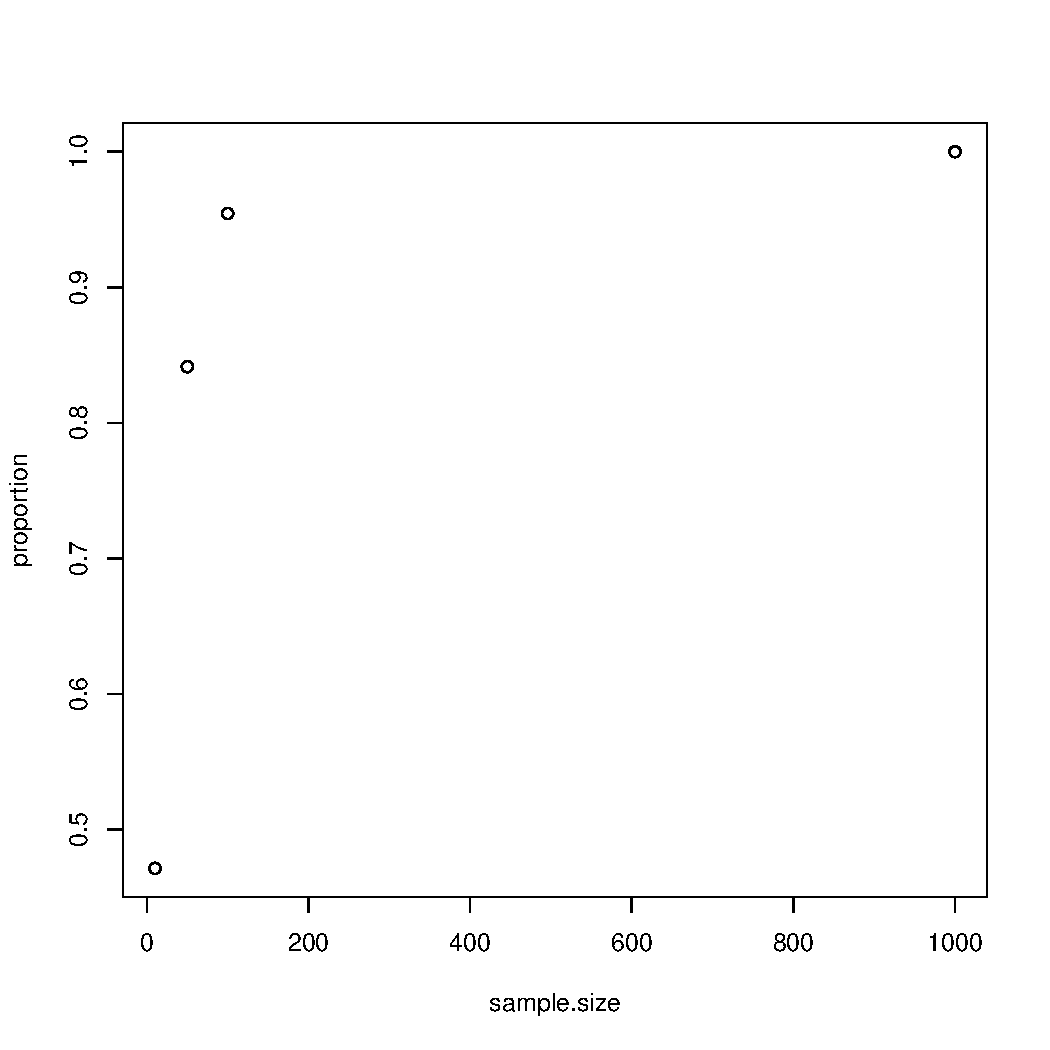
\includegraphics[width=\textwidth]{prob2_c.pdf}
	\end{center}
	There isn't much we can determine from this graph besides the fact that as the sample size goes 
	up, the proportion of diseased trees also goes up. The fact that at sample size 1000, we end up 
	with a proportion of 1, then this is most likely an error since it seems weird that we suddenly have 
	all diseased trees.

\clearpage
\section*{Problem 3} %%% DONE
\addsection{Third Problem}
% Answer on page 614.
% a. 99.8%, b. 99.5%, c. 85%, d. 68%

	\p{Exercise 7 in 7.2 on page 305} \mbox{} \\
	Assuming that $n$ is large, determine the confidence level for each of the following two-sided 
	confidence intervals: \\
	
	(a) $\bar{x} \pm \frac{3.09s}{\sqrt{n}}$\\
	(b) $\bar{x} \pm \frac{2.81s}{\sqrt{n}}$\\
	(c) $\bar{x} \pm \frac{1.44s}{\sqrt{n}}$\\
	(d) $\bar{x} \pm \frac{s}{\sqrt{n}}$ \\
	
	Note: the variable $z = \frac{(\bar{x}-\mu}{s/\sqrt{n}}$ also has approximately a standard normal 
	distribution. To solve each of these, we would just go to the Appendix Table 1 on pages 582-583 
	and use the $z$ values given as limits to the interval on the standard normal distribution so we 
	may find our confidence level.
	\addsubsection{Answer to 3.a}
	\p{Answer to a}
	\[ +3.09 = 0.999 \]
	\[ -3.09 = 0.001 \]
	\[ \text{difference } = 0.998 \]
	The confidence level for this two-sided confidence interval is 99.8\%.
	
	\addsubsection{Answer to 3.b}
	\p{Answer to b}
	\[ +2.81 = 0.9975 \]
	\[ -2.81 = 0.0025 \]
	\[ \text{difference } = 0.995 \]
	The confidence level for this two-sided confidence interval is 99.5\%.
	
	\addsubsection{Answer to 3.c}
	\p{Answer to c}
	\[ +1.44 = 0.9251 \]
	\[ -1.44 = 0.0749 \]
	\[ \text{difference } = 0.8502 \]
	The confidence level for this two-sided confidence interval is 85\%.
	
	\addsubsection{Answer to 3.d}
	\p{Answer to d}
	\[ +1.00 = 0.8413 \]
	\[ -1.00 = 0.1587 \]
	\[ \text{difference } = 0.6826 \]
	The confidence level for this two-sided confidence interval is 68.3\%.

\clearpage
\section*{Problem 4} %%% DONE Check answers
\addsection{Fourth Problem}

	\p{Exercise 8 in 7.2 on page 305} \mbox{} \\
	What $z$ critical value in the large-sample two-sided confidence interval for $\mu$ should be 
	used to obtain each of the following confidence levels? \\
	
	(a) 98\% \\
	(b) 85\% \\
	(c) 75\% \\
	(d) 99.9\% \\
	
	We can find each of these by multiplying the percentage by 100, adding 1 and then dividing by 
	two to get the value on the standard normal distribution table, and then doing a reverse lookup to 
	find the $z$ critical score.
	\addsubsection{Answer to 4.a}
	\p{Answer to a}
	\[ \frac{0.98+1}{2} = 0.99 \]
	Doing a reverse lookup in the table, we get a $z$ critical score of 2.33. Therefore:
	\[ \bar{x} \pm \frac{2.33s}{\sqrt{n}} \]
	
	\addsubsection{Answer to 4.b}
	\p{Answer to b}
	\[ \frac{0.85+1}{2} = 0.925 \]
	Doing a reverse lookup in the table, we get a $z$ critical score of 1.44. Therefore:
	\[ \bar{x} \pm \frac{1.44s}{\sqrt{n}} \]
	
	\addsubsection{Answer to 4.c}
	\p{Answer to c}
	\[ \frac{0.75+1}{2} = 0.875 \]
	Doing a reverse lookup in the table, we get a $z$ critical score of 1.15. Therefore:
	\[ \bar{x} \pm \frac{1.15s}{\sqrt{n}} \]
	
	\addsubsection{Answer to 4.d}
	\p{Answer to d}
	\[ \frac{0.999+1}{2} = 0.9995 \]
	Doing a reverse lookup in the table, we get a $z$ critical score of 3.29. Therefore:
	\[ \bar{x} \pm \frac{3.29s}{\sqrt{n}} \]

\clearpage
\section*{Problem 5} %%% DONE check answers
\addsection{Fifth Problem}
% Answer on page 614.
% a. Narrower, b. No, c. No, d. No

	\p{Exercise 11 in 7.2 on page 306} \mbox{} \\
	Suppose that a random sample of 50 bottles of a particular brand of cough syrup is selected, and 
	the alcohol content of each bottle is determined. Let $\mu$ denote the average alcohol content 
	for the population of all bottles of the brand under study. Suppose that the resulting 95\% 
	confidence interval is (7.8, 9.4). \\
	
	(a) Would a 90\% confidence interval calculated from this same sample have been narrower or 
	wider than the given interval? Explain your reason. \\
	(b) Consider the following statement: There is a 95\% chance that $\mu$ is between 7.8 and 9.4. 
	Is this statement correct? Why or why not? \\
	(c) Consider the following statement: We can be highly confident that 95\% of all bottles of this 
	type of cough syrup have an alcohol content that is between 7.8 and 9.4. Is this statement 
	correct? Why or why not?
	(d) Consider the following statement: if the process of selecting a sample size 50 and then 
	computing the corresponding 95\% interval is repeated 100 times, 95 of the resulting intervals will 
	include $\mu$. Is this statement correct? Why or why not?
	
	\addsubsection{Answer to 5.a}
	\p{Answer to a}
	The 90\% confidence interval calculated from this same sample would have been narrower than 
	the given interval since the formula we use to determine the interval, $\bar{x} \pm \frac{(z)(s)}
	{\sqrt{n}}$, depends on the $z$ critical value which is directly determined from the percentage of 
	the confidence interval, then the smaller confidence we have, the smaller the interval will be. The 
	price of a higher confidence level is a loss in precision.
	
	\addsubsection{Answer to 5.b}
	\p{Answer to b}
	No, this statement is not correct because a confidence level of 95\% implies that 95\% of all 
	samples would give an interval that includes $\mu$, while the above statement is saying that the 
	given interval will never change, which isn't true. The 95\% refers to the long-run percentage of 
	\emph{all} possible samples resulting in an interval that includes $\mu$.
	
	\addsubsection{Answer to 5.c}
	\p{Answer to c}
	No, this statement is not correct because the confidence level is just telling us what proportion of 
	samples have an interval that contains $\mu$ while the statement above is suggesting that the 
	confidence level is telling us the proportion of values that lie within an interval.
	
	\addsubsection{Answer to 5.d}
	\p{Answer to d}
	No, this statement is not correct because the 95\% confidence we are using refers to the long-run 
	percentage of \emph{all} possible samples resulting in an interval that includes $\mu$ and in this 
	statement, we only repeated the computation of the interval 100 times and not for every sample. 
	It is very likely that less or more than 95 of the samples will contain the correct interval.

\clearpage
\section*{Problem 6} %%% DONE
\addsection{Sixth Problem}
% For answer, check second edition: #15 on page 302
% a. (88.54, 89.66), b. 246

	\p{Exercise 16 in 7.2 on page 307} \mbox{} \\
	The article "Evaluating Tunnel Kiln Performance" (\emph{Amer. Ceramic Soc. Bull.}, August 1997: 
	59-63) gave the following summary information for fracture strengths (MPa) of $n=169$ ceramic 
	bars fired in a particular kiln: $\bar{x} = 89.10$, $s=3.73$. \\
	
	(a) Calculate a two-sided confidence interval for true average fracture strength using a 
	confidence level of 95\%. Does it appear that true average fracture strength has been precisely 
	estimated? \\
	(b) Suppose the investigators had believed a priori that the population standard deviation was 
	about 4 MPa. Based on this supposition, how large a sample would have been required to 
	estimate $\mu$ to within 0.5 MPa with 95\% confidence?
	
	\addsubsection{Answer to 6.a}
	\p{Answer to a}
	\[ \bar{x} \pm \frac{(z)(s)}{\sqrt{n}} \]
	Since we are dealing with a confidence level of 95\%, then we use the formula from problem 4 to 
	find the $z$ critical value of 1.96.
	\[ 89.10 \pm \frac{(1.96)(3.73)}{13} \]
	\[ (88.54, 89.66) \]
	
	\addsubsection{Answer to 6.b}
	\p{Answer to b}
	In order to solve this, the only thing we can really change is the sample size $n$. We want the 
	value we are adding and subtracting from $\bar{x}$ to be equal to 0.5, therefore:
	\[ 0.5 = \frac{(1.96)(4)}{\sqrt{n}} \]
	Solving for $n$, we get a sample size of 245.86, or 246 rounded up.
	
\section*{Problem 7} %%% DONE
\addsection{Seventh Problem}
% For answer, check second edition: # 17 on page 302
% a. 80%, b. 98%, c. 75%

	\p{Exercise 18 in 7.2 on page 307} \mbox{} \\
	Determine the confidence level for each of the following large-sample one sided confidence 
	bounds: \\
	
	(a) Upper bound: $\bar{x}+\frac{0.84s}{\sqrt{n}}$ \\
	(b) Lower bound: $\bar{x}-\frac{2.05s}{\sqrt{n}}$ \\
	(c) Upper bound: $\bar{x}+\frac{0.67s}{\sqrt{n}}$ \\
	
	To answer all of these questions, all we have to do is use the Appendix Table 1 on pages 582 and 
	583 and use the $z$ critical value to find the corresponding proportion.
	\addsubsection{Answer to 7.a}
	\p{Answer to a}
	Corresponding proportion to $z$ critical value of 0.84: \\
	0.7995 or 80\%.
	
	\addsubsection{Answer to 7.b}
	\p{Answer to b}
	Corresponding proportion to $z$ critical value of 2.05: \\
	0.9798 or 98\%.
	
	\addsubsection{Answer to 7.c}
	\p{Answer to c}
	Corresponding proportion to $z$ critical value of 0.67: \\
	0.7486 or 75\%.

\clearpage
\section*{Problem 8} %%% DONE
\addsection{Eighth Problem}
% Answer on page 614. #18 in second edition
% 390.74 min

	\p{Exercise 19 in 7.2 on page 307} \mbox{} \\
	The charge-to-tap time (min) for a carbon steel in one type of open hearth furnace was 
	determined for each heat in a sample of size 36, resulting in a sample mean time of 382.1 and a 
	sample standard deviation of 31.5. Calculate a 95\% upper confidence bound for true average 
	charge-to-tap time.
	
	\addsubsection{Answer to 8}
	\p{Answer}
	Since we are dealing with a confidence level of 95\%, then we use the table to find a $z$ critical 
	value of 1.645. To find the upper confidence bound, we would use the formula:
	\[ \bar{x} + \frac{(z)(s)}{\sqrt{n}} \]
	\[ 382.1 + \frac{(1.645)(31.5)}{\sqrt{36}} \]
	\[ 390.73625 \]
	With a confidence level of 95\%, the value of $\mu$ lies in the interval (0, 390.74) min. Since we 
	can't have a negative charge-to-tap time, then the lower bound was changed to 0.

\section*{Problem 9} %%% DONE
\addsection{Ninth Problem}
% Answer on page 614.
% a. (0.50, 0.56) We are 99% confident the proportion of all adult Americans who have watched streamed programming is between 50% and 56%., b. 664

	\p{Exercise 23 in 7.3 on page 315} \mbox{} \\
	TV advertising agencies face growing challenges in reaching audience members because 
	viewing TV programs via digital streaming is increasingly popular. The Harris poll reported on 
	November 13, 2012, that 53\% of 2343 American adults surveyed said they have watched 
	digitally streamed TV programming on some type of device. \\
	
	(a) Calculate and interpret a confidence interval at the 99\% confidence level for the proportion of 
	all adult Americans who have watched streamed programming. \\
	(b) What sample size would be required for the width of a 99\% CI to be at most 0.05 irrespective 
	of the value of $p$?
	
	\addsubsection{Answer to 9.a}
	\p{Answer to a}
	In order to calculate this, we will use the formula $p \pm (z\text{ critical value })\sqrt{p(1-p)/n}$ 
	where $p=0.53$, $z=2.576$, and $n=2343$.
	\[ 0.53 \pm 2.576\sqrt{\frac{0.53(1-0.53)}{2343}} \]
	\[ (0.50, 0.56) \]
	Given the above interval, we are 99\% confident the proportion of all adult Americans who 
	watched streamed programming is between about 50\% and 56\%.
	
	\addsubsection{Answer to 9.b}
	\p{Answer to b}
	We will solve this problem in a similar way we solved problem 6.b. We just set 
	$2.576\sqrt{\frac{0.53(1-0.53)}{n}}$ equal to 0.05 and then solve for $n$. By doing this, we get a 
	sample size of 662.

\clearpage
\section*{Problem 10} %%% DONE check answer with someone else
\addsection{Tenth Problem}

	\p{Exercise 30 in 7.3 on page 317} \mbox{} \\
	A manufacturer of small appliances purchases plastic handles for coffeepots from an outside 
	vendor. If a handle is cracked, it is considered defective and must be discarded. A very large 
	shipment of handles is received. The proportion of defective handles, $\pi$, is of interest. How 
	many handles from the shipment should be inspected to estimate $\pi$ to within 0.1 with 99\% 
	confidence?
	
	\addsubsection{Answer to 10}
	\p{Answer}
	In order to answer this question, we must use the formula
	\[ n = \pi(1-\pi)\left[\frac{z}{B}\right]^2 \]
	Where $n$ is the sample size, $z$ is the $z$ critical score, $\pi$ is the proportion of defective 
	handles received which is going to be equal to 0.5 since $\pi(1-\pi)$ is largest when $\pi=0.5$, 
	and $B$ is the bound which equals 0.1 in this case.
	\[ n = 0.5(0.5)\left[\frac{2.576}{0.1}\right]^2 \]
	\[ n = 165.8944 \]
	Round up to the nearest integer and we get $n = 166$.
	
\end{document}